\section{System Architecture and Modules}
The FM Radio receiver is designed as a high-performance streaming pipeline. Data flows from the input I/Q samples through a series of filtering and transformation stages summarized in Fig.~\ref{fig:block_diagram}.

\begin{figure}[H]
    \centering
    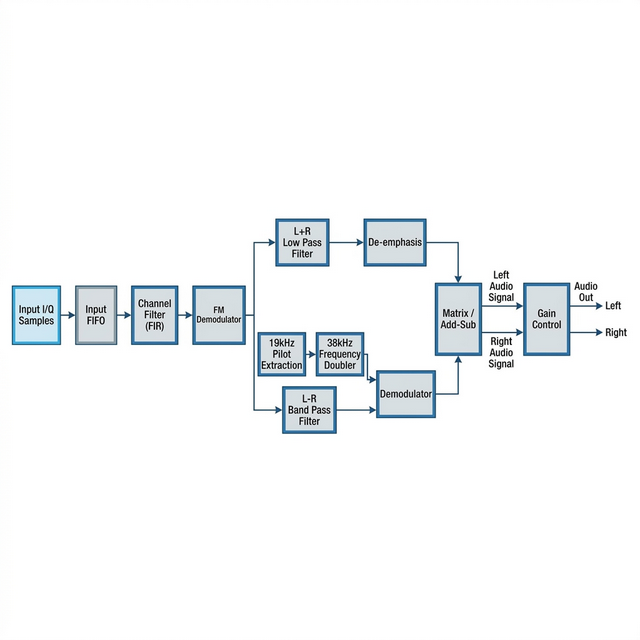
\includegraphics[width=\textwidth]{images/block_diagram.png}
    \caption{System Architecture of the FM Stereo Radio Receiver}
    \label{fig:block_diagram}
\end{figure}

\subsection{System Parameters}
The hardware implementation is strictly aligned with the software reference model specifications:
\begin{itemize}
    \item \textbf{Sampling Rate}: Input USRP rate of 256 kHz (\texttt{QUAD_RATE}), decimated by 8 to 32 kHz (\texttt{AUDIO_RATE}) for audio output.
    \item \textbf{Quantization}: 10-bit fixed-point precision (\texttt{QUANT_VAL = 1024}), using Q10 format for all internal arithmetic.
    \item \textbf{Demodulation Gain}: Approximately 758 (Q10), calculated as $\frac{\text{QUAD\_RATE}}{2\pi \times 55000} \times 1024$.
\end{itemize}

\subsection{Phase 1: Channel Filtering and Demodulation}
The front end of the receiver extracts the baseband FM signal from the USRP raw data.

\subsubsection{Complex Channel Filter}
The input USRP data is first passed through a 20-tap Complex Low-Pass Filter (cutoff 80 kHz). In our hardware implementation, since the imaginary coefficients are zero, this is realized by instantiating two parallel 20-tap real FIR modules (\texttt{fir.sv}) processing the I and Q channels independently.

\subsubsection{FM Demodulator (\texttt{demodulate.sv})}
The demodulator computes the instantaneous frequency. It first performs a conjugate multiplication $I[n] + jQ[n] \cdot (I[n-1] - jQ[n-1])$ to find the phase difference. The angle is then extracted using a \textbf{Quad-Arctan} algorithm, which uses a piecewise rational approximation instead of CORDIC:
\begin{align*}
    \text{if } x \ge 0: & \quad r = \frac{x - |y|}{x + |y|}, \quad \text{angle} = \frac{\pi}{4} - \frac{\pi}{4}r \\
    \text{if } x < 0: & \quad r = \frac{x + |y|}{|y| - x}, \quad \text{angle} = \frac{3\pi}{4} - \frac{\pi}{4}r
\end{align*}
Hardware realization utilizes a 32-stage pipelined restoring divider to compute the ratio $r$ at high frequency.

\subsection{Phase 2: Stereo Separation and Reconstruction}
The demodulated signal is split into three parallel paths:

\subsubsection{Mono Path ($L+R$)}
A 32-tap LPF (cutoff 15 kHz) extracts the mono component. This module performs the 8x decimation, outputting samples at 32 kHz.

\subsubsection{Pilot Path (38 kHz Carrier Generation)}
A 32-tap BPF extracts the 19 kHz pilot tone. The tone is then squared to generate a second-harmonic component (38 kHz + DC). A final 32-tap High-Pass Filter removes the DC component, providing a clean 38 kHz carrier synchronized with the station.

\subsubsection{Stereo Difference Path ($L-R$)}
A 32-tap BPF (23-53 kHz) captures the DSB-SC modulated $L-R$ signal. This is multiplied by the 38 kHz carrier to perform down-conversion back to baseband, followed by another 32-tap LPF and 8x decimation.

\subsection{Phase 3: Final Matrixing and Post-Processing}
The synchronized $L+R$ and $L-R$ signals are combined via addition and subtraction to yield raw $L$ and $R$ channels.

\subsubsection{De-emphasis and Gain}
FM broadcasting uses pre-emphasis (boosting high frequencies) to improve SNR. Our hardware reverses this using a 1st-order IIR de-emphasis filter (\texttt{deemphasis.sv}) with a $75 \mu s$ time constant. The final audio signal is scaled using a parameterizable gain module (\texttt{gain.sv}) before output.
